\documentclass{standalone}
\usepackage{tikz}
\usepackage{ctex,siunitx}
\setCJKmainfont{Noto Serif CJK SC}
\usepackage{tkz-euclide}
\usepackage{amsmath}
\usetikzlibrary{patterns, calc,3d}
\usetikzlibrary {decorations.pathmorphing,decorations.pathreplacing,decorations.shapes}
\begin{document}
\small
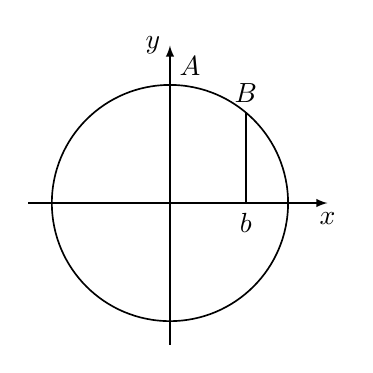
\begin{tikzpicture}[>=latex,scale=1.0]
  \draw[->](-1.8,0)--(2.0,0)node[below]{$x$};
  \draw[->](0,-1.8)--(0,2.0)node[left]{$y$};
  \draw[semithick](0,0)circle(1.5);
  \node at(0,1.5)[above right]{$A$};
  \draw[semithick](50:1.5)node[above]{$B$}--({1.5*cos(50)},0)node[below]{$b$};
\end{tikzpicture}
\end{document}